\section{Cray Application Level Placement Scheduler (ALPS)}

\begin{figure*}
  \centering
  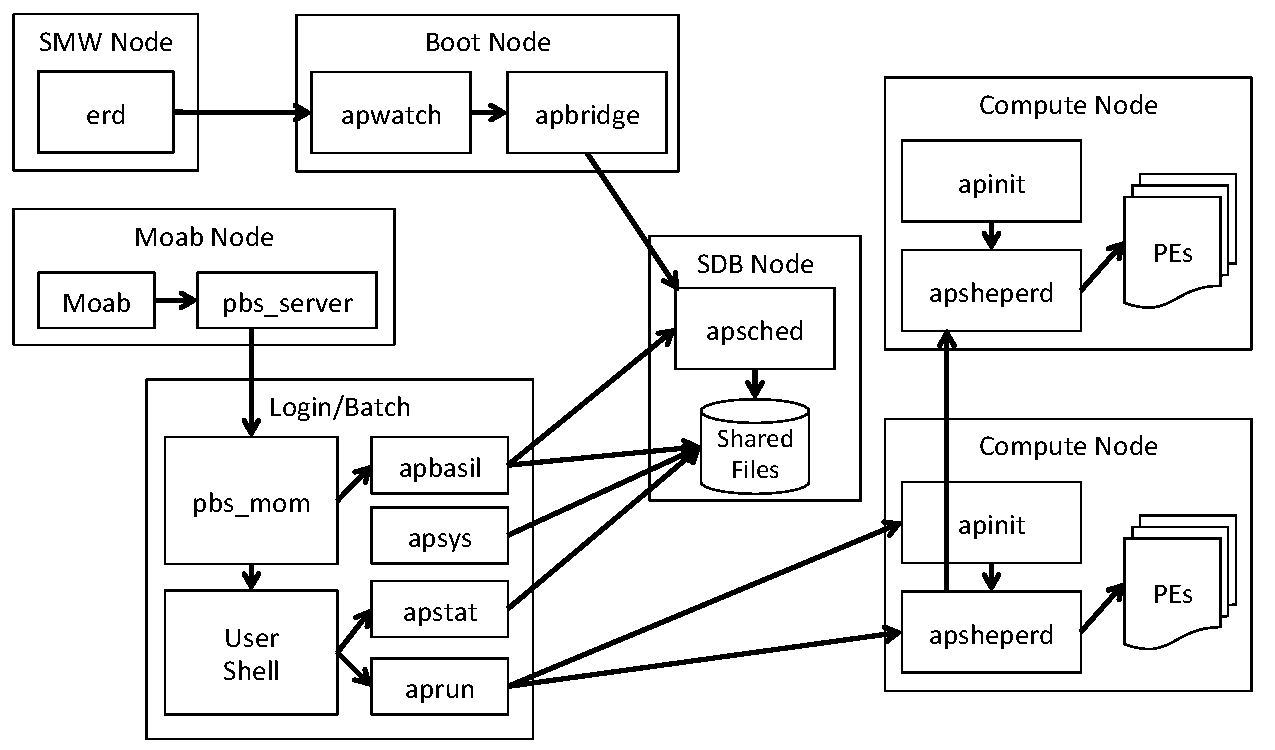
\includegraphics[width=6.5in]{figures/alps-hilevel.pdf}\\
  \caption{High-Level ALPS Design}\label{fig:alps-hilevel}
\end{figure*}

The term ``resource manager'' is overloaded in the batch processing world, and
the combination of systems needed to effectively control batch processing on
the Cray X-series platform certainly supports the confusion.  At the lowest
level in the Cray hierarchy sits the Cray Application Level Placement Scheduler,
commonly referred to as ALPS \cite{alps}.  While in most instances, a batch
system is making scheduling decisions based upon configuration of center
policy, ALPS is the piece of software at the lowest level that is handed
information from the batch system to ultimately launch the job onto the compute
nodes.

Not only does ALPS launch jobs, it maintains compute node state and
reservations to manage job placement and resource utilization.  Through a
series of daemons that typically run on the Cray boot or system database (sdb)
node, ALPS imports hardware configuration information from the system database
to provide memory, CPU and GPU resources available on each compute node.  Given
a heterogeneous system, this would be essential to providing the user with a
mechanism to request the resources needed to run a particular application.
Each compute node also has a state and mode associated with it that informs
ALPS whether the node is up or down and whether it is in interactive or batch
mode.  Up and down states are self-explanatory, and there are a few other
states that will not be discussed that are in the end classified as up or down,
but interactive or batch mode requires some explanation.  

ALPS can operate without a batch system sitting at a higher level providing
information.  This is called interactive mode, and it is basically a FIFO queue
that requires users to run ALPS commands that sit and wait for available
resources to run jobs.  How is this different from a batch system?  In a
nutshell, batch systems provide a mechanism for the user to submit a job to be
run at a later time without the burden of making sure the machine doesn't
reboot taking the waiting ALPS command down with it. Batch systems also allow a
priority-based reordering of jobs based on policies determined by the center.
In contrast, batch mode simply enables the use of a batch system for job launch
ignoring any user-supplied ALPS commands run outside of the batch system.

Reservations are used to manage availability of nodes that are in an up state.
When a job is launched, it is assigned to a set of nodes. Those nodes are
exclusively reserved for that job.  When the job finishes, the reservation is
destroyed, and those nodes are available for the next job.  Reservations are
simply the mechanism by which a job receives exclusive access to the resources
necessary to run the job.

All of the ALPS information must somehow get communicated to the batch system
in order to provide the user with the available resources on the system and to
maintain a consistent state for nodes, reservations, and jobs.  ALPS provides
an API called \emph{apbasil} - BASIL being an acronym for Batch Application
Scheduler Interface Layer.  BASIL is an XML-based protocol that provides batch
systems with the ability to retrieve inventories of compute nodes, their states
and reservations, and the ability to create, confirm, and delete reservations.
Using this interface, batch systems are able to manage all aspects of job
submission, scheduling, placement and deletion by communicating with ALPS which
communicates directly with the compute nodes.
